\chapter{前言}
\renewcommand{\baselinestretch}{10.0} %設定行距
\pagenumbering{arabic} %設定頁號阿拉伯數字
\setcounter{page}{1}  %設定頁數
\fontsize{14pt}{2.5pt}\sectionef
\section{整體架構}
    經過討論後,我們將整個BubbleRob分為三大主題,分別為 「 SolidWorks 」 、「 CoppeliaSim 」 、「 Lua 」,再分數個小主題去完成本次競賽。下圖為本次競賽整體架構(圖.\ref{fig.機器人報告表格})\\

\begin{figure}[hbt!]
\begin{center}
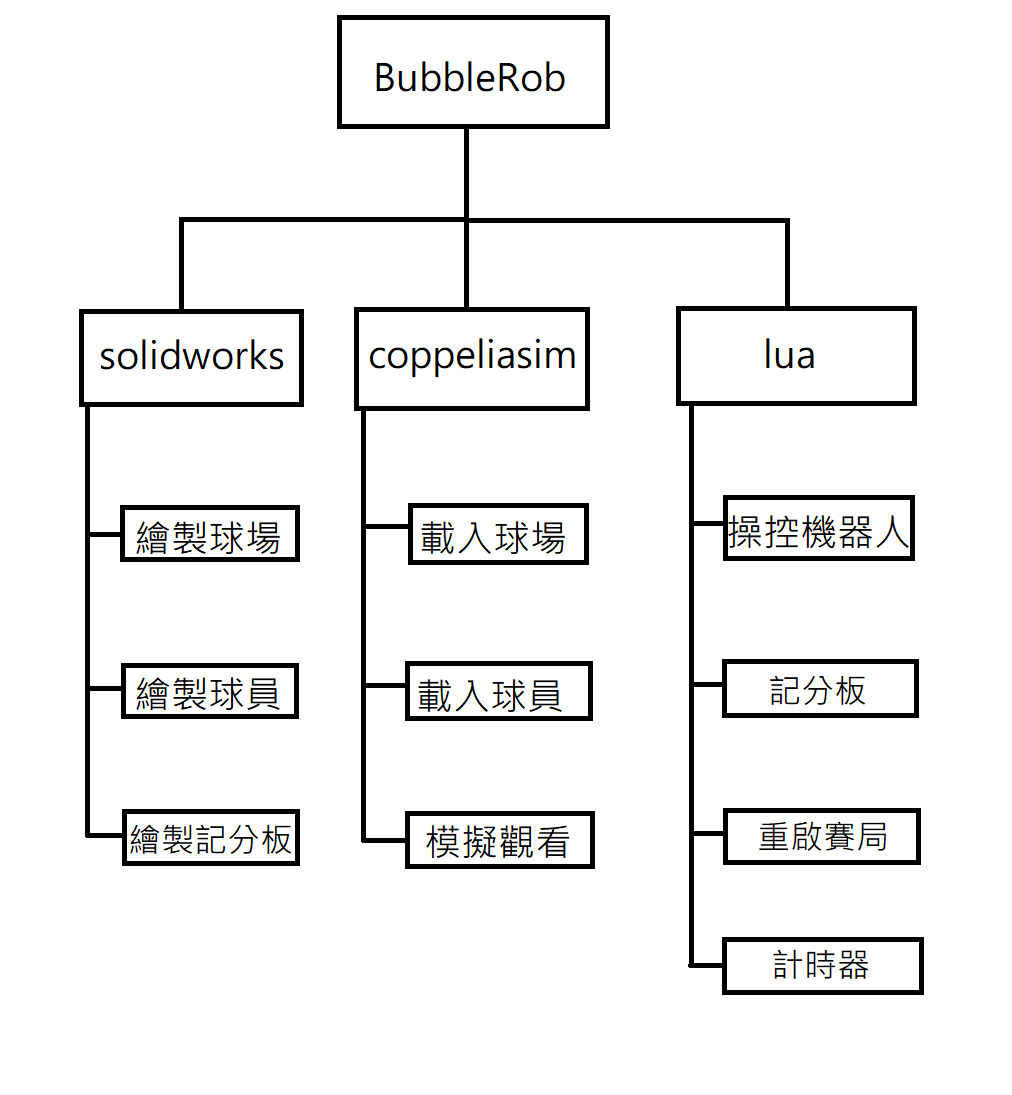
\includegraphics[width=13cm]{機器人報告表格}
\caption{\Large 心智圖}\label{fig.機器人報告表格}
\end{center}
\end{figure}


\section{規則說明}
類似於手足球,一開始時球會置於場中央,遊戲開始後兩方在不同地點連上同一個網路即可
以鍵盤操控機器人推球至已方的球門得分。\\
 
遊戲規則如下:\\

\begin{center}
    足球觸碰到球門感測器即算得分\\
    在限時內得越多分數的隊伍即獲勝\\
    任一方進球得分後,球員的位置不變,球會回到場中央重新開始\\
\end{center}
\begin{figure}[hbt!]
\begin{center}
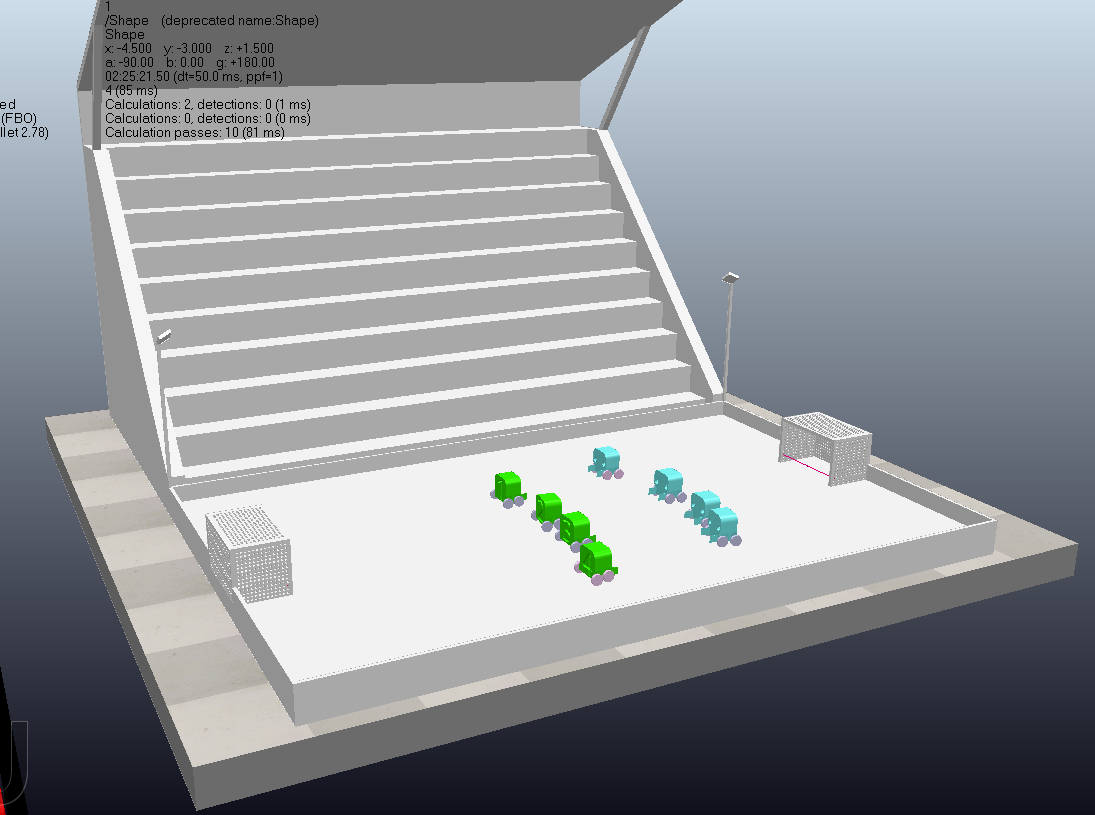
\includegraphics[width=15cm]{機器人報告2}
\caption{\Large 機器人報告2 }
\label{機器人報告2 }
\end{center}
\end{figure}

\renewcommand{\baselinestretch}{0.5} %設定行距